\section{Data}
\subsection{Study frame and charging measures}
The study combines city-week charging records with local policy documents for 2016--2023. A registry of 334 Chinese cities fixes the spatial frame, and a crosswalk links original city names to provinces and administrative identifiers. Its 2,672 city-year cells distinguish unobserved outcomes from observed charging records. Policy coverage is recorded independently, allowing each comparison to use the observations appropriate to its question rather than a single complete-case panel.

The charging data comprise 139,612 city-week observations from one anonymized operator network made available with \citet{ma2026}. We use the second release of these data, which describes the operator's observed network rather than a census of public charging. Activity is analyzed on its reported scale because the available documentation does not establish its physical unit. The cumulative facility indicator measures observed facility scale; its correspondence to stations, piles or connectors is not established, and it does not measure instantaneous operating capacity. Source versions and measurement metadata are documented in SI Section~\siref{sec:si-sources}.

A compatible week has a valid source date and positive cumulative facilities. Within each city $i$ and annual or quarterly period $t$, $W_{it}$ counts compatible weeks, $Q_{it}$ sums their activity, and $E_{it}$ sums their cumulative-facility values over the same dates. The resulting measures are
\begin{equation}
A_{it}=Q_{it}/W_{it},\qquad N_{it}=E_{it}/W_{it},\qquad I_{it}=A_{it}/N_{it}=Q_{it}/E_{it}.
\label{eq:metrics}
\end{equation}
Thus $A$ is activity per compatible week, $N$ is mean observed facilities, and $I$ is activity relative to facilities. The cumulative facility indicator is used directly; stock is not reconstructed from installation records. Normalization aligns exposure across observed dates without assuming that missing weeks resemble observed weeks.

Compatible weeks with zero activity remain in the measures. A period with $W>0,Q=0$ is source-coded zero; no compatible weeks yields missing ratios. The source does not consistently distinguish inactivity, reporting and anonymization. Coverage is $W/W^{\mathrm{cal}}$, using the source calendar's 53 dates in 2017 and 2023 and 52 otherwise. Positive-record frequency $p=W^+/W$ and positive-week mean activity $q^+$ describe the internal composition of recorded activity. Table~\ref{tab:sources} reports the distributions on their stated supports.
\begin{table}[htbp]\centering\small\setlength{\tabcolsep}{4.5pt}\caption{Measurement and descriptive statistics}\label{tab:sources}
\begin{tabular}{@{}p{35mm}p{27mm}rrrrr@{}}\toprule
Measure and source scale & Sample & City-years / cities & P25 & Median & P75 & P95\\
\midrule
Facilities $N$\par facility-indicator units & Facility-observable & 890 / 293 & 4.00 & 12.67 & 53.04 & 796.00\\
Activity $A$\par source units/week & Facility-observable & 890 / 293 & 0.00 & 2.02 & 8,527.92 & 313,682.66\\
Activity $A$\par source units/week & Positive activity & 464 / 123 & 454.06 & 6,829.25 & 52,282.63 & 564,777.99\\
Intensity $I$\par source units/(facility-week) & Facility-observable & 890 / 293 & 0.00 & 0.13 & 202.65 & 958.48\\
Intensity $I$\par source units/(facility-week) & Positive activity & 464 / 123 & 15.47 & 185.84 & 542.85 & 1,203.74\\
Compatible weeks $W$\par weeks & Facility-observable & 890 / 293 & 42.00 & 52.00 & 53.00 & 53.00\\
\bottomrule\end{tabular}\end{table}


\subsection{Policy linkage and contextual measures}
Local policy documents originate in the multi-level energy-transition corpus and its registered release \citep{zhaopaper2026,zhao2026}. City applicability, document identifiers, issuing authorities, dates and coverage status determine linkage. Unknown coverage remains distinct from documented absence of a qualifying requirement. Policy dates retain their available precision, with interval rules for quarterly comparisons; clause functions describe prescribed responsibilities rather than observed compliance. Source selection, matching and clause coding are specified in SI Section~\siref{sec:si-sources} and SI Section~\siref{sec:si-policy}.

Daily NASA POWER weather at representative city points provides annual temperature, degree-day, precipitation, wind and humidity measures \citep{nasapower}. Annual charging models use five weather controls, whereas annual policy models use four. Quarterly models use no weather because no quarterly series is available. Provincial pandemic-response records are matched by province and source date \citep{hale2021}. Their index measures policy response, with coverage ending in February 2023; matched model comparisons therefore stop in 2022, without filling later values.

\subsection{Coverage and analytical use}
Facilities are observed in 890 city-years across 293 cities: 464 rows in 123 cities have positive activity and 426 have source-coded-zero activity. The other 1,782 registry cells have no compatible weeks. Facility-observable coverage grows from 18 cities in 2016 to 293 in 2023, while positive-activity coverage grows from 13 to 114. These changes describe archive coverage. Fixed-city comparisons separate longitudinal growth from this expansion of the observation frame.

Facility scale also varies substantially: its median is \FacilityMedian\ and mean \FacilityMean\ across observable city-years. The quarterly frame contains 10,688 city-quarters, of which 3,083 have compatible facilities: 1,551 positive-activity and 1,532 coded-zero rows. Annual and quarterly model supports apply the eligibility rules in Methods, with period-specific details in SI Section~\siref{sec:si-annual} and SI Section~\siref{sec:si-quarterly}. Descriptive fixed-window memberships instead follow endpoint or continuous-window requirements.

Administrative-code matching locates 333 study-city polygons among 372 geographical features, leaving one registry name unmatched. Figure~\ref{fig:coverage} places the observed network within this geography; maps identify cities rather than service catchments. Figure~\ref{fig:observation} retains all 334 registry cities in its coverage display and uses variable-specific positive supports for log distributions. Together, coverage and scale determine what each city count, distribution and network aggregate represents.
\begin{figure}[htbp]\centering
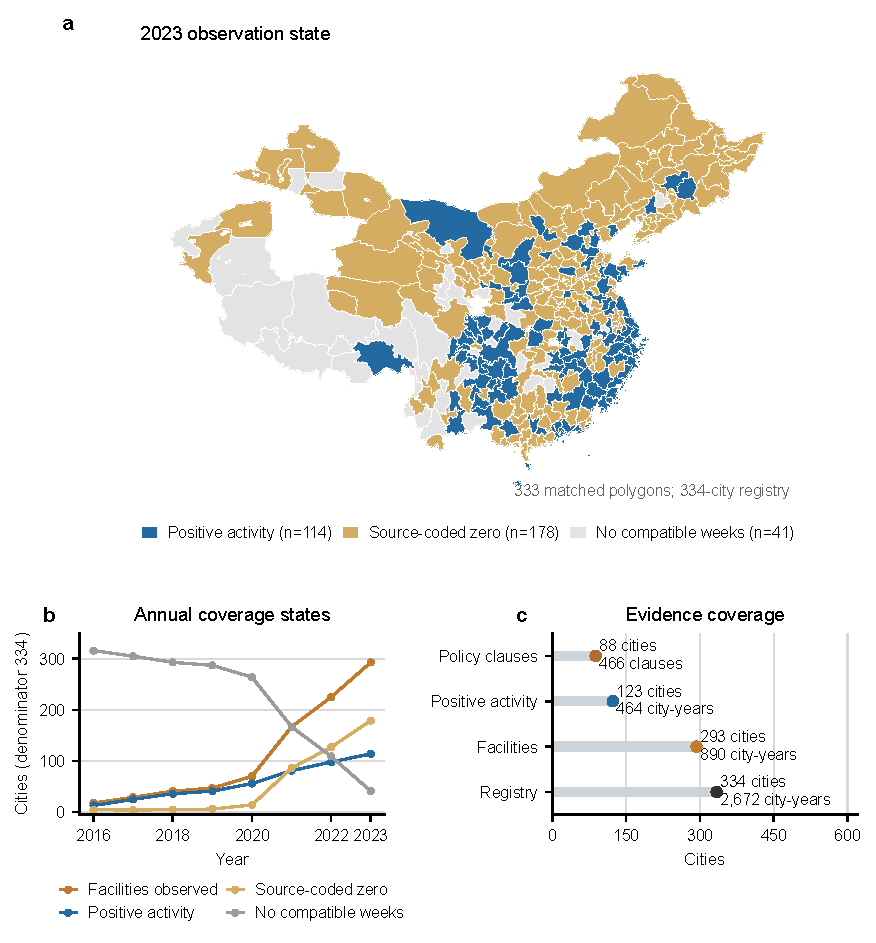
\includegraphics[width=\linewidth,height=.76\textheight,keepaspectratio]{figures/fig1_coverage.pdf}
\caption{Spatial and temporal data coverage}\label{fig:coverage}
\end{figure}

\begin{figure}[htbp]\centering
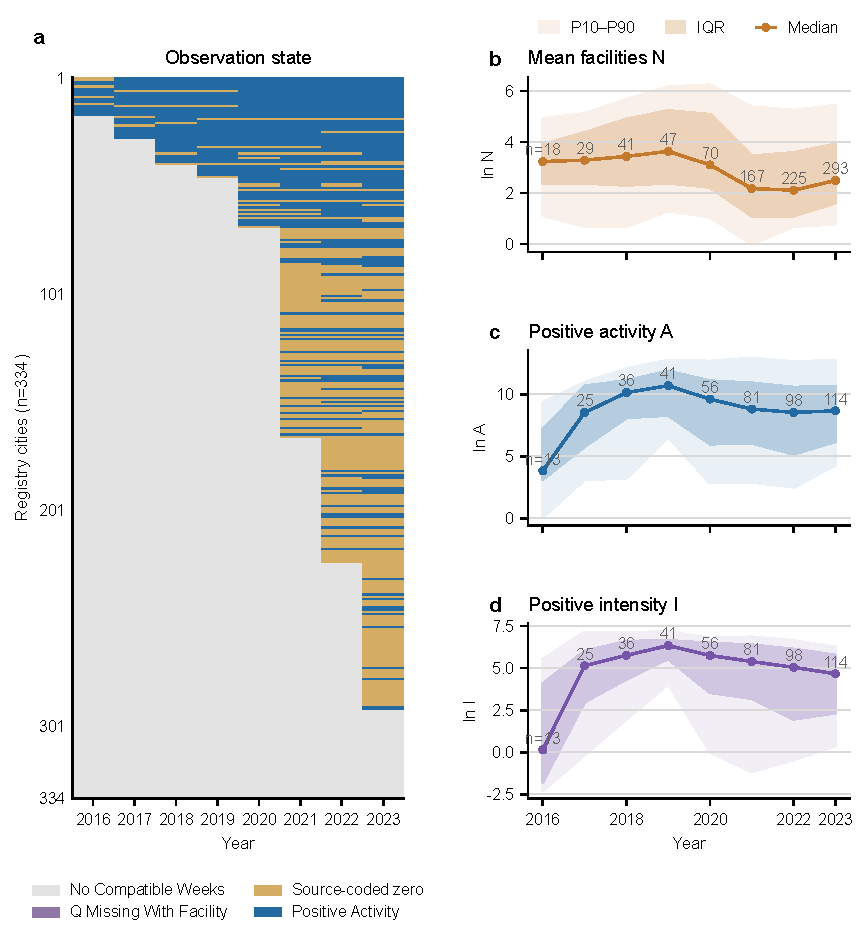
\includegraphics[width=\linewidth,height=.76\textheight,keepaspectratio]{figures/fig2_observation.pdf}
\caption{Observation patterns and outcome distributions}\label{fig:observation}
\end{figure}

